% !TEX TS-program = lualatex
% !TEX encoding = UTF-8 Unicode		

\documentclass[12pt, letterpaper]{article}

%%BIBLIOGRAPHY- This uses biber/biblatex to generate bibliographies according to the 
%%Unified Style Sheet for Linguistics
\usepackage[main=american, german]{babel}% Recommended
\usepackage{csquotes}% Recommended
\usepackage[backend=biber,
		style=unified,
		maxcitenames=3,
		maxbibnames=99,
		natbib,
		url=false]{biblatex}
\addbibresource{link_laptop.bib}
\setcounter{biburlnumpenalty}{100}  % allow URL breaks at numbers
%\setcounter{biburlucpenalty}{100}   % allow URL breaks at uppercase letters
%\setcounter{biburllcpenalty}{100}   % allow URL breaks at lowercase letters

%%TYPOLOGY
\usepackage[svgnames]{xcolor} % Specify colors by their 'svgnames', for a full list of all colors available see here: http://www.latextemplates.com/svgnames-colors
%\usepackage[compact]{titlesec}
%\titleformat{\section}[runin]{\normalfont\bfseries}{\thesection.}{.5em}{}[.]
%\titleformat{\subsection}[runin]{\normalfont\scshape}{\thesubsection}{.5em}{}[.]
\usepackage[hmargin=1in,vmargin=1in]{geometry}  %Margins          
\usepackage{graphicx}	%Inserting graphics, pictures, images 		
\usepackage{stackengine} %Package to allow text above or below other text, Also helpful for HG weights 
\usepackage{fontspec} %Selection of fonts must be ran in XeLaTeX or LuaLaTeX
\usepackage{amssymb} %Math symbols
\usepackage{amsmath} % Mathematical enhancements for LaTeX
\usepackage{setspace} %Linespacing
\usepackage{multicol} %Multicolumn text
\usepackage{enumitem} %Allows for continuous numbering of lists over examples, etc.
\usepackage{multirow} %Useful for combining cells in tablesbrew 
\usepackage{booktabs}
\usepackage{hanging}
\usepackage{fancyhdr} %Allows for the 
\pagestyle{fancy}
\fancyhead[L]{\textit{290 Entrance Paper}} 
\fancyhead[R]{\textit{\today}} 
\fancyfoot[L,R]{} 
\fancyfoot[C]{\thepage} 
\renewcommand{\headrulewidth}{0.4pt}
\setlength{\headheight}{14.5pt} % ...at least 14.49998pt
% \usepackage{fourier} % This allows for the use of certain wingdings like bombs, frowns, etc.
% \usepackage{fourier-orns} %More useful symbols like bombs and jolly-roger, mostly for OT
\usepackage[colorlinks,allcolors={black},urlcolor={blue}]{hyperref} %allows for hyperlinks and pdf bookmarks
% \usepackage{url} %allows for urls
% \def\UrlBreaks{\do\/\do-} %allows for urls to be broken up
\usepackage[normalem]{ulem} %strike out text. Handy for syntax
\usepackage{tcolorbox}
\usepackage{datetime2}

%%FONTS
\setmainfont{Libertinus Serif}
\setsansfont{Libertinus Sans}
\setmonofont[Scale=MatchLowercase]{Libertinus Mono}

%%PACKAGES FOR LINGUISTICS
%\usepackage{OTtablx} %Generating tableaux with using TIPA
% \usepackage[noipa]{OTtablx} % Use this one generating tableaux without using TIPA
%\usepackage[notipa]{ot-tableau} % Another tableau drawing packing use for posters.
% \usepackage{linguex} % Linguistic examples
% \usepackage{langsci-linguex} % Linguistic examples
\usepackage{langsci-gb4e} % Language Science Press' modification of gb4e
% \usepackage{langsci-avm} % Language Science Press' AVM package
\usepackage{tikz} % Drawing Hasse diagrams
\usetikzlibrary{positioning}
% \usepackage{pst-asr} % Drawing autosegmental features
% \usepackage{pstricks} % required for pst-asr, OTtablx, pst-jtree.
% \usepackage{pst-jtree} 	% Syntax tree draawing software
% \usepackage{tikz-qtree}	% Another syntax tree drawing software. Uses bracket notation.
\usepackage{forest}	% Another syntax tree drawing software. Uses bracket notation.
% \usepackage{ling-macros} % Various linguistic macros. Does not work with linguex.
% \usepackage{covington} % Another linguistic examples package.
\usepackage{leipzig} %	Offers support for Leipzig Glossing Rules

%%LEIPZIG GLOSSING FOR ZAPOTEC
\newleipzig{eld}{eld}{elder}				% Elder pronouns
\newleipzig{hum}{hum}{human}				% Human pronouns
\newleipzig{ani}{ani}{animate}			% Animate pronouns
\newleipzig{ina}{ina}{inanimate}			% Inanimate pronouns
\newleipzig{pot}{pot}{potential}		% Potential Aspect
\newleipzig{cont}{cont}{continuative}	% Continuative Aspect
\newleipzig{stat}{stat}{stative}		% Stative Aspect
\newleipzig{and}{and}{andative}			% Andative Aspect
\newleipzig{ven}{ven}{venative}			% Venative Aspect
\newleipzig{rest}{rest}{restitutive}	% Restitutive Aspect
\newleipzig{rep}{rep}{repetitive}		% Repetitive Aspect

%%TITLE INFORMATION
\title{TITLE}
\author{Mykel Loren Brinkerhoff}
\date{\today}

%%MACROS
\newcommand{\sub}[1]{\textsubscript{#1}}
\newcommand{\supr}[1]{\textsuperscript{#1}}
\providecommand{\lsptoprule}{\midrule\toprule}
\providecommand{\lspbottomrule}{\bottomrule\midrule}
\newcommand{\fittable}[1]{\resizebox{\textwidth}{!}{#1}}

\makeatletter
\renewcommand{\paragraph}{%
  \@startsection{paragraph}{4}%
  {\z@}{0ex \@plus 1ex \@minus .2ex}{-1em}%
  {\normalfont\normalsize\bfseries}%
}
\makeatother
\parindent=10pt


\begin{document}
	
%%If using linguex, need the following commands to get correct LSA style spacing
%% these have to be after  \begin{document}
	% \setlength{\Extopsep}{6pt}
	% \setlength{\Exlabelsep}{9pt}		%effect of 0.4in indent from left text edge
%%
	
%% Line spacing setting. Comment out the line spacing you do not need. Comment out all if you want single spacing.
%	\doublespacing
	\onehalfspacing
	
\begin{center}
	{\Large \textbf{Interaction of tone and phonation in Santiago Laxopa Zapotec}}
	\vspace{6pt}

	Mykel Loren Brinkerhoff
\end{center}
%\maketitle
%\maketitleinst
\thispagestyle{fancy}

% \tableofcontents

%------------------------------------
\section{Introduction} \label{sec:Introduction}
%------------------------------------

The interaction between tone and phonation is primarily believed to consist of phonation being closely linked with certain tones depending on the language under discussion \citep{yipTone2002,weePhonologicalTone2019}. This has lead to a growing body of literature that assumes this to be a universal fact about tonal languages (\citet{michaudComplexTonesEast2012,brunelleTonePhonationSoutheast2016,hymanToneSystems2020,garellekPhoneticsWhiteHmong2021} among many others). This, however, is not true for languages of the Americas. One of the linguistic areas where tone and phonation do not seem to be closely tied to one another is in Mesoamerica \citep{campbellMesoAmericaLinguisticArea1986,silvermanLaryngealComplexityOtomanguean1997,campbellOtomangueanHistoricalLinguistics2017a,campbellOtomangueanHistoricalLinguistics2017}. \citet{silvermanLaryngealComplexityOtomanguean1997} shows how tone and phonation are truly decoupled and result in a ``laryngeally complex" system. 

One of these languages that shows laryngeal complexity is Santiago Laxopa Zapotec, an Oto-Manguean language spoken in Oaxaca, Mexico. As will be discussed in Section \ref{sec:SLZ}, Santiago Laxopa Zapotec has a system of four phonation types and five tones which allows for a detailed study into how such systems are produced. 

My qualifying paper will explore the interaction of tone and phonation in Santiago Laxopa Zapotec which will add to our understanding of how such laryngeally complex system are produced. This investigation will be based on data that I have collected from two native Santiago Laxopa Zapotec speakers that live in Santa Cruz, CA. Additionally, I will explore how best to represent such systems using the Laryngeal Articulator Model \citep{eslingVoiceQualityLaryngeal2019}. The Laryngeal Articulator Model is a model which takes into account the full complexity of the lower vocal tract by using a series of monovalent states. The Laryngeal Articulator Model is described in more detail in Section~\ref{sec:LAM}.  

%------------------------------------
\section{Tone and Phonation} \label{sec:TonePhonation}
%------------------------------------

Tone, as a linguistic phenomenon, is very wide spread and is present in many of the world's languages \citep{yipTone2002}. Most of the tonal languages that have received the most attention are languages from Africa and Asia with languages of the Americas receiving some attention \citep{pikeToneLanguagesTechnique1948,silvermanLaryngealComplexityOtomanguean1997,campbellOtomangueanHistoricalLinguistics2017a,campbellOtomangueanHistoricalLinguistics2017}. Because of the focus on mostly African and Asian tonal languages certain assumptions are commonly held about what is possible for tonal languages. One of the assumptions that is made is that tone and phonation are heavily dependent on each other \citep{andruskiPhonationTypesProduction2000,yipTone2002,garellekVoiceQualityTone2013,brunelleTonePhonationSoutheast2016,weePhonologicalTone2019,hymanToneSystems2020,garellekPhoneticsWhiteHmong2021}. For example, Mandarin tone three, which is produced as a dipping tone in careful speech and a falling tone in rapid speech, has creakiness throughout the vowel. This creakiness is often the sole clue to differentiate it from a normal falling tone \citep{duanmuPhonologyStandardChinese2007,kuangCovariationVoiceQuality2017}. 

Oto-Manguean languages from Mexico clearly show that the behavior between tone and phonation in Asia is not the only way in which tone and phonation can interact. In fact, Oto-Manguean languages have what \citet{silvermanLaryngealComplexityOtomanguean1997} calls ``laryngeally complex'' vowels. These laryngeally ccomplex vowels are ones where tone and phonation are entirely independent from one another. This means that any tone can co-occur with any phonation type. Some work has been done that adequately shows this such as \citet{avelinobecerraTopicsYalalagZapotec2004,chavez-peonInteractionMetricalStructure2010,dicanioCoarticulationToneGlottal2012,uchiharaToneRegistrogenesisQuiavini2016}. One of the more detailed of these studies is \citet{chavez-peonInteractionMetricalStructure2010} who investigates the phonetic cues to tone, stress, and phonation in San Lucas Quiaviní Zapotec (SLQZ) a Valley Zapotec variety. \citeauthor{chavez-peonInteractionMetricalStructure2010} shows how tone and phonation are mostly independent from each other with a notable exception being the restriction of Rising tone in SLQZ which can only appear with modal phonation. The distribution of tone and phonation type is presented in Table \ref{tab:slqz}.

\begin{table}[!ht]
\centering
\caption{SLQZ tone and phonation}
\label{tab:slqz}
 \begin{tabular}{lcccc}
  \lsptoprule
  				&	 High  & Low & Falling & Rising \\
  	Modal	& ✔︎ & ✔︎ & ✔︎ & ✔︎ \\
  	Breathy & X & ✔︎ & ✔︎ & X \\
  	Creaky & ✔︎ & ✔︎ & ✔︎ & X \\
  	Interrupted & ✔︎ & ✔︎ & ✔︎ & X \\
  \lspbottomrule
 \end{tabular}
\end{table}

My qualifying paper will add to this lesser studied area of phonetics and phonology by investigating the interaction of tone and phonation in Santiago Laxopa Zapotec.

%------------------------------------
\section{Overview of Santiago Laxopa Zapotec} \label{sec:SLZ}
%------------------------------------

Santiago Laxopa Zapotec (SLZ) is a variety of Sierra Norte Zapotec, a member of the Oto-Manguean language family, and spoken by approximately 800 to 1200 people in the municipality of Santiago Laxopa, Oaxaca, Mexico \citep{adlerDerivationVerbInitiality2018,sichelPronounsAttractionSierra2020}. Similar to other Oto-Manguean languages, SLZ exhibits \citeauthor{silvermanLaryngealComplexityOtomanguean1997}'s (\citeyear{silvermanLaryngealComplexityOtomanguean1997}) ``larnygeally complex vowels''. In addition to its five-vowel inventory, SLZ makes further distinctions with the addition of breathy, checked,\footnote{There are two ways in which this vowel can be analyzed. One is the traditional way where the glottal stop is considered inseparable from the vowel. The other is to treat this as a consonant which is restricted to only reside in codas (similar to how the sound /ŋ/ is restricted to codas in English). This second approach is the one taken by \citet{avelinobecerraTopicsYalalagZapotec2004}. I will follow the traditional way of analyzing these vowels through this paper.} and laryngealized\footnote{Previous descriptions of the the vowel system of closely related languages have used various different terms for this vowel including broken, rearticulated, interrupted, and creaky \citep{longDiccionarioZapotecoSan2005,avelinoAcousticElectroglottographicAnalyses2010,avelinobecerraTopicsYalalagZapotec2004,sonnenscheinDescriptiveGrammarSan2005,adlerAcousticsPhonationTypes2016}. In order to avoid confusion, I will use the term laryngealized following \citet{avelinoAcousticElectroglottographicAnalyses2010}.} phonations. The different phonation types are also represented in the orthography for SLZ as seen in (\ref{ex:phonation})
\ea \label{ex:phonation}
	Breathy: [ a̤ ] <\textit{ah}> \\
	Checked: [ aˀ ] <\textit{a'}> \\
	Laryngealized: [ aˀa ] <\textit{a'a}> \\
\z
There are many words that are differentiated by only by phonation in SLZ. For example, the words for \emph{snake} and \emph{fish} are only distinguished by the presence of breathy phonation, (\ref{ex:SnakeFish}). 

\ea \label{ex:SnakeFish}
	\ea \textit{behl} [ bɛ̤lː¹³ ] `snake'
	\ex \textit{bel} [ bɛlː¹³ ]`fish'
	\z  
\z 

In addition to phonation, SLZ, along with all of the Oto-Manguean languages, is a tonal language \citep{brinkerhoffDownstepSantiagoLaxopaMFM}. SLZ has three level tones of high, mid, and low, which are represented in the transcriptions with Pike's numbers, where x¹ is the highest tone and x³ is the lowest \citep{pikeToneLanguagesTechnique1948,weePhonologicalTone2019}. In addition to these three level tones, SLZ has two contour tones, a rising (x²¹) and a falling tone (x¹³). The number of tones were discovered by myself and two other researchers following the methods for tonal analysis in \citet{pikeToneLanguagesTechnique1948,sniderToneAnalysisField2018}. An overview of the different tonal patterns are seen in Table \ref{tab:tones}.

\begin{table}[!h]
\centering
\caption{SLZ tones}
\label{tab:tones}
 \begin{tabular}{lllll}
  \lsptoprule
  				% &	 Diacritic  & Example & Transcription \\
  High   	&  a¹  &  \textit{xha}   &  [ ʐa¹ ] & `clothing.\textsc{poss}'\\
	Mid    	&  a²  &  \textit{lhill} 	& [ ɾiʒ² ] & `house.\textsc{poss}' \\
	Low   	&  a³  &  \textit{yu'} 	&	 [ çuˀ³ ] & `earth'\\
	Rising	&  a²¹  &  \textit{yu'u} 	&	[ juˀu²¹ ] & `quicklime (Sp. cal)' \\
	Falling &  a¹³  &  \textit{yu'u}  &	[juˀu¹³] &	`house' \\
  \lspbottomrule
 \end{tabular}
\end{table}

SLZ sits at an important crossroads of studying tone and phonation because it is a language that has both independent tone and phonation. This combination allows for a thorough investigation into how tone and phonation interact which is an area that is still not well understood. Additionally, SLZ allows for us to investigate the phonetic realization of phonological contrasts. 

%------------------------------------
\section{Methods and materials} \label{sec:Methods}
%------------------------------------

In order to investigate what is occurring with SLZ tone and phonation, two SLZ speakers, who live in Santa Cruz, CA, were asked to produce approximately 200 words in SLZ in a carrier sentence three times. This allowed for a good overlap between tone and phonation type. Because data collection occurred during the COVID-19 pandemic two methods were used to elicit data. The first was using Zencastr\footnote{\href{https://zencastr.com/}{https://zencastr.com/}}, a professional podcasting website, to prevent potential exposure to each other. Once we were all vaccinated and it was deemed safe by myself and my consultants, we meet at in the backyard of the consultants and recording was done using a Zoom H4n audio recorder (44.1kh-16bit).  

\ea Carrier Sentence \label{ex:carrier}\\
\gll sh-ni=a'¹³ \rule{10mm}{1pt} cho²ne² las²\\ 
\textsc{cont}-speak=1\textsc{sg} \rule{10mm}{1pt} three times\\
\trans `I say \rule{10mm}{1pt} three times'	
\z 

Once the recordings were made, the audio files were initially segmented using ELAN \citep{wittenburgELANProfessionalFramework2006} and then passed to PRAAT \citep{boersmaPraatDoingPhonetics2021} for segmenting the vowels and extracting them for analysis in VOICESAUCE \citep{shueVOICESAUCEProgramVoice2009}.I am currently segmenting the vowels out of the audio files in PRAAT and will shortly be analyzing the extracted vowels in VOICESAUCE. 

%------------------------------------
\section{Laryngeal Articulator Model} \label{sec:LAM}
%------------------------------------

One way that the interaction between phonation and tone could be understood is with \citeauthor{eslingVoiceQualityLaryngeal2019}'s (\citeyear{eslingVoiceQualityLaryngeal2019}) Laryngeal Articulator Model. The Laryngeal Articulator Model takes as a basic assumption that laryngeal articulations are more complex than what most phonological feature systems represent. For example the feature system in \citet{hayesIntroductoryPhonology2009} assumes that only three features ([± voice], [± constricted glottis], and [± spread glottis]) are able to capture the full range of laryngeal complexity. This, however, is a gross simplification of the articulation in the larynx. For breathy voice because the larynx is open, the airflow is less turbulent and less impeded allowing for more linear airflow through the pharyngeal space \citep[56]{eslingVoiceQualityLaryngeal2019}. Creaky voice on the other hand is produced with thick, short vocal folds. Additionally, a loose aspect is required which is thyroarytenoid muscles from the borders of the arytenoids to the front of the epilaryngeal tube \citet[63]{eslingVoiceQualityLaryngeal2019}. However, the ventricular folds can couple with the vocal folds during creaky phonation. This coupling has four effects: (i) it increases the overall effective vibrating mass, lowering frequency; (ii) it adds damping, making vibration more likely to cease; (iii) it adds increased degrees of freedom to the system, encouraging irregular vibration; and, most importantly, (iv) it perturbs the transmission of the mucosal wave by preventing its traversal across the surface of the vocal folds, causing the wave energy to be reflected back towards the midline earlier than what would occur for modal phonation \citep[63]{eslingVoiceQualityLaryngeal2019}. 

Based on these complexities in the lower vocal tract that accompany laryngeal and pharyngeal, \citeauthor{eslingVoiceQualityLaryngeal2019} propose their Laryngeal Articulator Model which attempts to capture the `articulatory' realization of the larynx following \citet{ohalaPhoneticExplanationsSound2005,ohalaAccommodationAerodynamicVoicing2011}. In accounting for the physiological states that the lower vocal tract is in during speech production, \citeauthor{eslingVoiceQualityLaryngeal2019} propose the addition of a network of synergistic and anti-synergistic physiological relations that are represented in the Figure~\ref{fig:LAMNetwork}.

\begin{figure}[!ht]
\caption{Network of synergistic and anti-synergistic physiological relations among vocal tract states}
\label{fig:LAMNetwork}
\centering
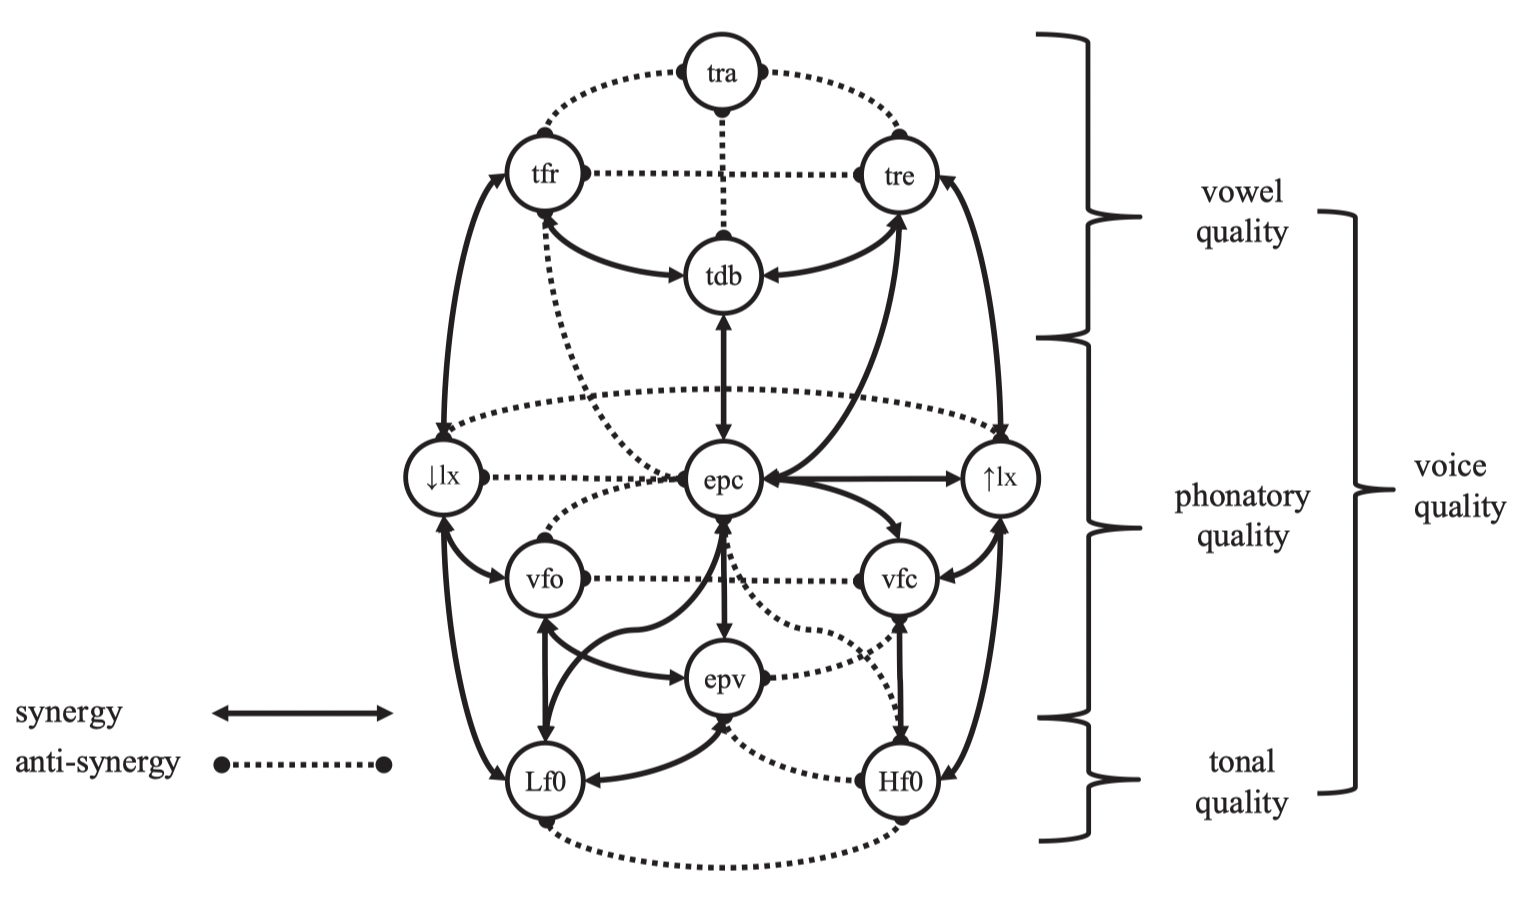
\includegraphics[width=0.9\textwidth]{LAMNetwork.png}
\end{figure}

\begin{table}[!ht]
\centering
\caption{Physiological states of the lower vocal tract}
\label{tab:States}
 \begin{tabular}{ll}
  \lsptoprule
  States	&	 Physiological description \\
  \hline
  vfo   	&  vocal folds open (abducted) \\
	vfc    	&  vocal folds closed (adducted/prephonation)\\
	epc   	&  epilaryngeal constriction\\
	epv			&  epilaryngeal vibration \\
	tfr 		&  tongue fronting \\
	tre 		&  tongue retraction \\
	tra 		&  tongue raising \\
	tdb 		&	 tongue double bunching\\
	↑lx     &  raised larynx\\
	↓lx			&  lowered larynx\\
	Hf0			&  increased vocal fold tension, less vibrating mass (high f0)\\
	Lf0			&  decreased vocal fold tension, more vibrating mass (lower f0)\\
  \lspbottomrule
 \end{tabular}
\end{table}

Using these networks, one can more accurately describe what is occurring in the larynx during phonation. I plan on using these networks to describe and account for the the interaction between tone and phonation in SLZ. 

%------------------------------------
\section{Conclusion} \label{sec:Conclusion}
%------------------------------------

This paper has laid out our current understanding of the interaction of tone and phonation and what is possible. Additionally, our current understanding of the tone and phonation in SLZ was described. I also provided a description of the methods that I am employing to investigate this interaction. One potential way of explaining the complex interactions of tone and phonation could potentially be found in the Laryngeal Articulator Model was also introduced. 

%------------------------------------
%BIBLIOGRAPHY
%------------------------------------

%\singlespacing
%\nocite{*}
\printbibliography[heading=bibintoc]

\end{document} 